\documentclass{article}
\usepackage{xeCJK}
\usepackage{graphicx}
\usepackage{fancyhdr}
\date{}
\usepackage{geometry}
\usepackage{hyperref}
\usepackage{multirow}
\usepackage{float}
\usepackage[figurename=图,tablename=表]{caption}


\geometry{a4paper, margin=1in}
\title{《中山大学农业与生物技术学院导师双选系统》}
\author{性能测试报告}

\begin{document}

\maketitle

\section*{一、压力测试}
本次性能测试的目标是评估系统在高并发情况下的性能表现,旨在确保系统在实际使用中能够承载较大的流量和负载。经过此次测试,发现系统已经具备较为稳定的性能表现,能够在较高并发下正常使用,且没有出现重大异常问题,表明系统基本达到预期性能标准并可投入使用。

\subsection*{1.测试环境}
网络:2500Mbps局域网 \\
设备:AMD7950x 16核心32线程、64G DDR5内存 \\
操作系统:Windows 10专业版 \\
测试时间:2024年10月15日下午2点 \\
测试协议:HTTP/HTTPS \\
测试地址:\url{https://select.lumoxuan.cn}

\subsection*{2. 测试场景}
测试主要针对三个接口进行模拟:
\begin{itemize}
    \item \textbf{GET /hello}:用于测试系统的基本连通性。
    \item \textbf{POST /api/auth/login}:用于测试用户登录功能。
    \item \textbf{GET /student/teachers}:用于测试学生查询导师列表功能。
\end{itemize}

测试共设置了三个HTTP请求采样器,并配置了如下线程组参数:
\begin{itemize}
    \item \textbf{线程数}:100
    \item \textbf{Ramp-up时间}:100秒
    \item \textbf{持续时间}:600秒
\end{itemize}
(模拟了100名用户同时访问网站,持续十分钟的情况,模拟了系统可能承载的最大压力)

\subsection*{3. 测试结果}
测试过程中,每秒大约有87个请求发出,系统的平均响应时间约为1.05秒,整体吞吐量和响应时间都维持在较为平稳的状态。具体性能指标如下:

\subsubsection*{1. 响应时间}
响应时间是指系统从接收到请求到返回响应的时间。理想情况下,响应时间应保持在较低范围内,以确保用户体验良好。在本次测试中,平均响应时间为1.05秒。

\subsubsection* {2. 吞吐量}
吞吐量(Throughput)是指系统每秒处理的请求数,吞吐量越高,系统的处理能力越强。本次测试的吞吐量为87.2请求/秒。

\subsubsection* {3. 错误率}
错误率是指请求失败的比例。在本次测试中,系统的错误率为0.00%,表明所有请求均成功处理。

\subsubsection*{主要性能指标}
\begin{itemize}
    \item \textbf{平均响应时间}:约1.05秒
    \item \textbf{90\% 分位数响应时间}:2.2秒
    \item \textbf{99\% 分位数响应时间}:2.8秒
    \item \textbf{最大响应时间}:5.4秒
    \item \textbf{吞吐量}:87.2请求/秒
    \item \textbf{错误率}:0.00\%
\end{itemize}

\subsubsection*{图形展示}
\begin{figure}[H]
    \centering
    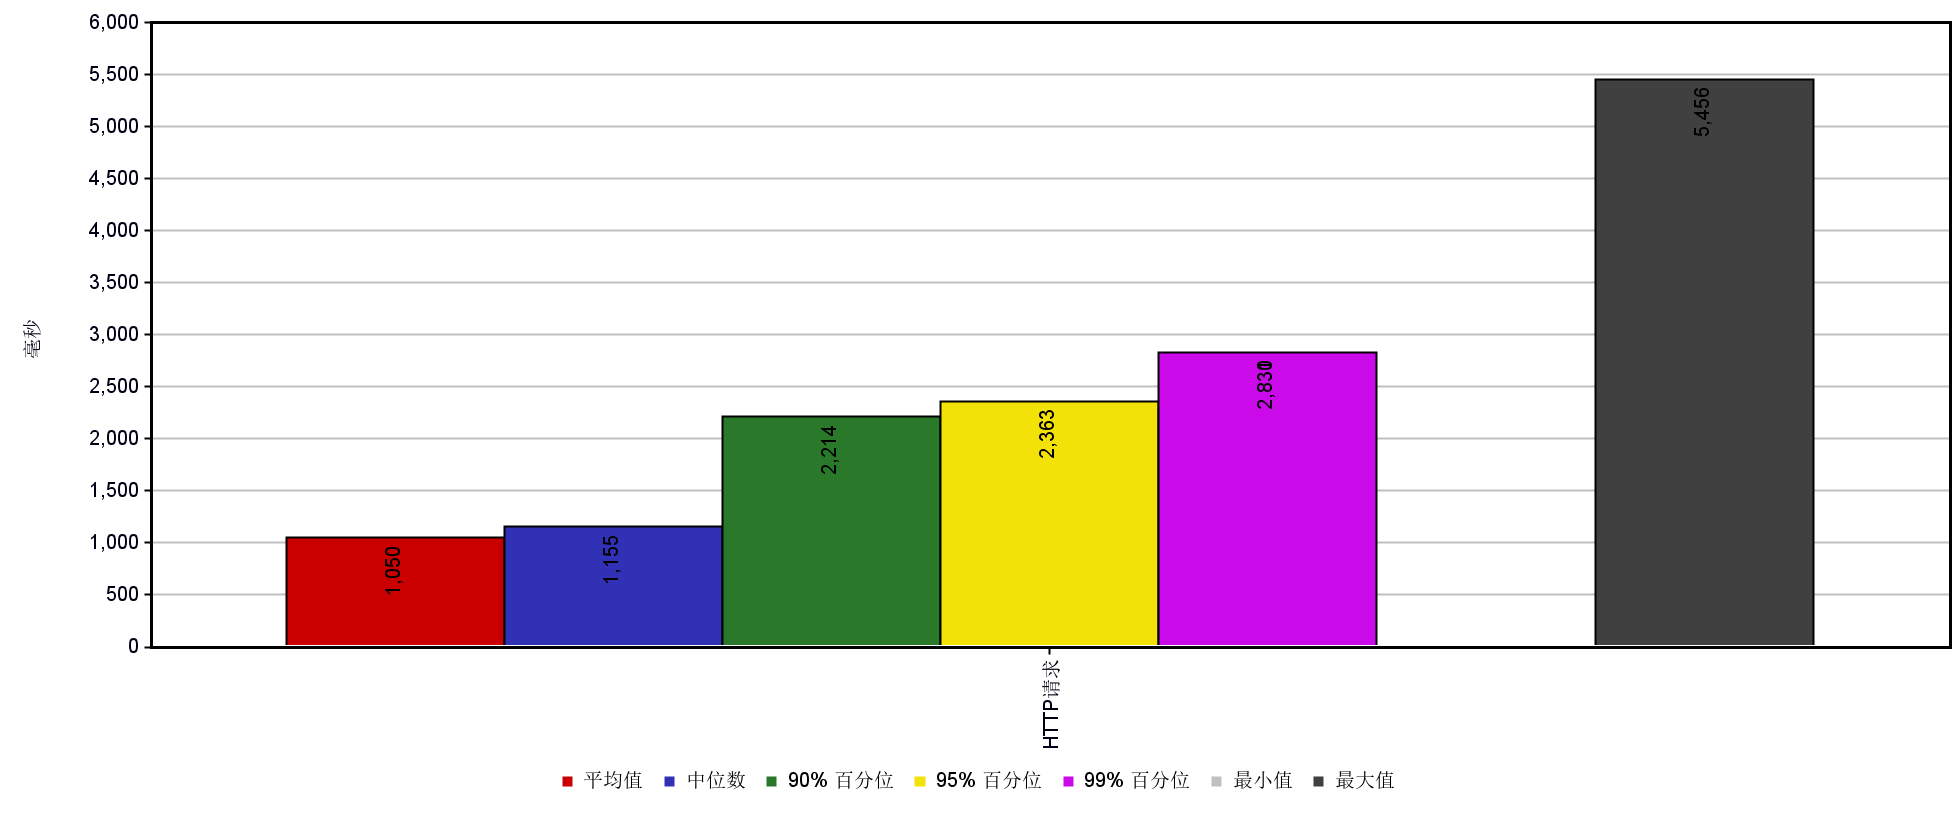
\includegraphics[width=1\textwidth]{result_image.png}
    \caption{性能测试汇总图}
\end{figure}

测试结果显示,系统在高并发条件下大部分请求的响应时间在1到2秒之间,只有少数请求的响应时间超过了5秒,这些表现可以认为是合理的。

\section*{二、网站速度诊断}

为了进一步验证系统的可用性,我们使用了ITDOG工具对系统的访问速度进行了测试,分别进行了两类测速:
\begin{itemize}
    \item \textbf{缓慢测速}:模拟的是正常环境下的网站访问速度,多个节点在正常情况下对系统进行测试,以获取较为真实的响应速度。
    \item \textbf{快速测速}:模拟的是在高并发环境下的访问速度,116个测速节点同时进行并发访问,测试系统在高负载压力下的响应速度。
\end{itemize}

这两种测试方法可以帮助我们更好地理解系统在不同负载条件下的表现,确保系统在正常使用和高并发情况下都能稳定运行。

\subsection*{2.1 快速测速结果}
快速测速模拟了116个节点同时并发访问系统的情况,目的是测试系统在高并发压力下的响应速度。以下是快速测速的结果展示:

\begin{figure}[H]
    \centering
    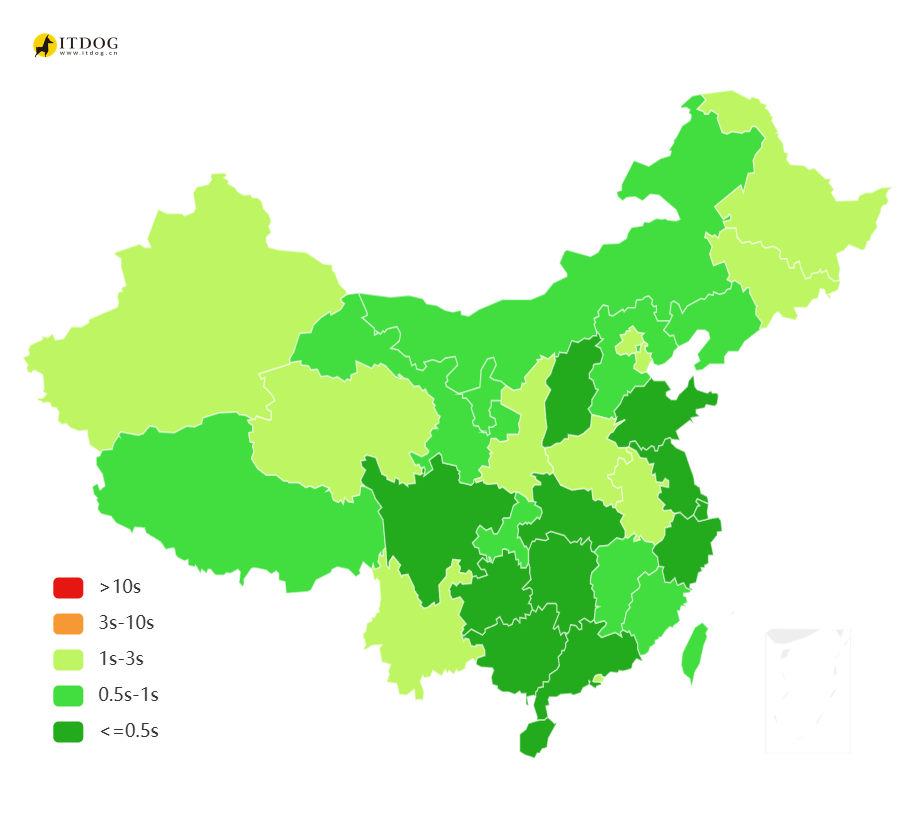
\includegraphics[width=0.8\textwidth]{快速测速.png}
    \caption{快速测速图}
\end{figure}

\begin{table}[H]
    \centering
    \begin{tabular}{|l|l|l|l|}
        \hline
        \textbf{区域/运营商} & \textbf{最快} & \textbf{最慢} & \textbf{平均} \\ \hline
        全部节点 & 江西南昌联通 0.136s & 广东广州电信 2.22s & 1.243s \\ \hline
        中国电信 & 上海电信 0.272s & 广东广州电信 2.220s & 1.168s \\ \hline
        中国联通 & 江西南昌联通 0.136s & 内蒙古联通 1.852s & 1.254s \\ \hline
        中国移动 & 浙江杭州移动 0.304s & 新疆乌鲁木齐移动 1.895s & 1.316s \\ \hline
        华东地区 & 江西南昌联通 0.136s & 安徽阜阳电信 2.002s & 1.063s \\ \hline
        华南地区 & 海南海口电信 0.496s & 广东广州电信 2.220s & 1.306s \\ \hline
        华中地区 & 湖北武汉电信 0.407s & 河南郑州电信 1.825s & 0.933s \\ \hline
        华北地区 & 天津移动 0.875s & 河北承德移动 1.853s & 1.353s \\ \hline
        西南地区 & 重庆电信 0.506s & 云南昆明移动 1.837s & 1.277s \\ \hline
        西北地区 & 陕西西安联通 0.582s & 新疆乌鲁木齐移动 1.966s & 1.256s \\ \hline
        东北地区 & 辽宁大连电信 1.189s & 吉林长春电信 2.054s & 1.720s \\ \hline
        港澳台 & 中国台湾 1.077s & -- & 1.304s \\ \hline
    \end{tabular}
    \caption{快速测速表格}
\end{table}

\subsection*{2.2 缓慢测速结果}
缓慢测速模拟的是正常环境下的单个节点访问系统的情况,测试系统在无高并发压力时的响应速度,结果如下:

\begin{figure}[H]
    \centering
    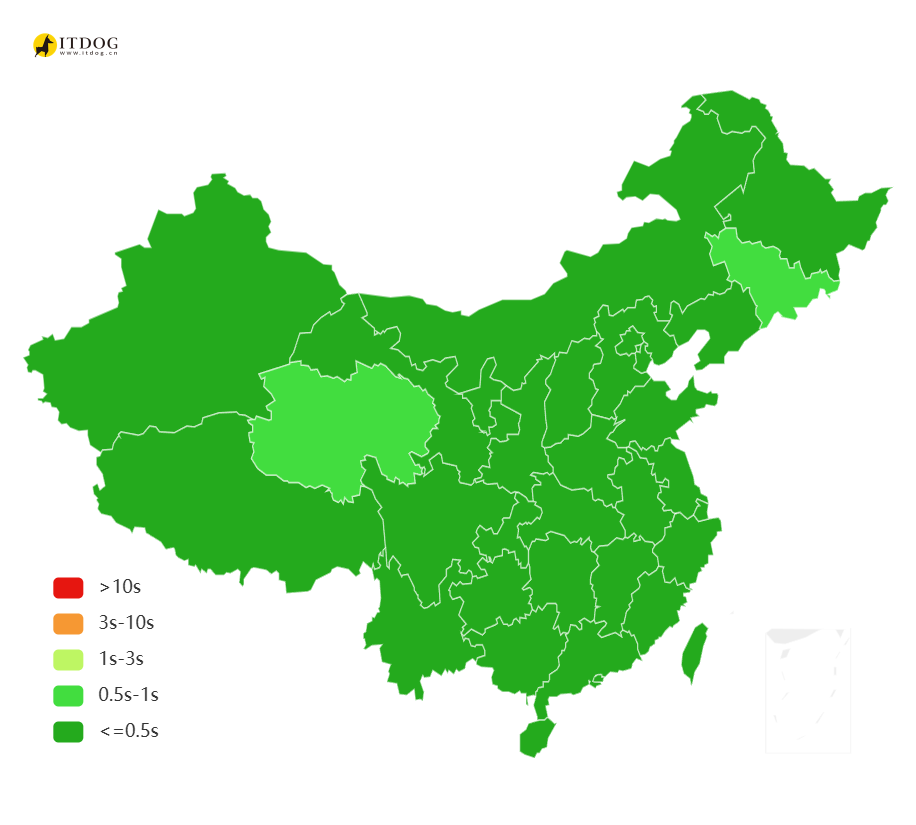
\includegraphics[width=0.8\textwidth]{缓慢测速.png}
    \caption{缓慢测速图}
\end{figure}

\begin{table}[H]
    \centering
    \begin{tabular}{|l|l|l|l|}
        \hline
        \textbf{区域/运营商} & \textbf{最快} & \textbf{最慢} & \textbf{平均} \\ \hline
        全部节点 & 江西南昌联通 0.111s & 上海电信 3.133s & 0.394s \\ \hline
        中国电信 & 广东广州电信 0.183s & 上海电信 3.133s & 0.438s \\ \hline
        中国联通 & 江西南昌联通 0.111s & 黑龙江哈尔滨联通 0.895s & 0.351s \\ \hline
        中国移动 & 江西南昌移动 0.136s & 湖南长沙移动 1.432s & 0.382s \\ \hline
        华东地区 & 江西南昌联通 0.111s & 上海电信 3.133s & 0.392s \\ \hline
        华南地区 & 广东广州电信 0.183s & 广西南宁移动 0.662s & 0.266s \\ \hline
        华中地区 & 湖北武汉移动 0.173s & 河南洛阳电信 2.016s & 0.537s \\ \hline
        华北地区 & 北京电信 0.205s & 河北邯郸联通 0.571s & 0.341s \\ \hline
        西南地区 & 重庆移动 0.207s & 云南昆明移动 0.550s & 0.358s \\ \hline
        西北地区 & 陕西西安电信 0.198s & 新疆乌鲁木齐移动 0.782s & 0.434s \\ \hline
        东北地区 & 辽宁大连移动 0.321s & 黑龙江哈尔滨联通 0.895s & 0.465s \\ \hline
        港澳台 & 中国台湾 0.350s & -- & 0.459s \\ \hline
    \end{tabular}
    \caption{缓慢测速表格}
\end{table}

\section*{三、结论}
经过多项测试,包括压力测试和网站访问速度诊断,我们得出以下结论:
\begin{itemize}
    \item 系统整体性能良好,能够在高并发情况下正常运行,具有良好的响应时间和稳定性。
    \item 在快速测速中,系统的响应速度较为理想,能够满足用户日常访问的需求。
    \item 在缓慢测速中,虽然存在高并发压力,但系统依然保持了稳定的响应,且平均响应时间依然在可接受范围内。
\end{itemize}

总体而言,系统在各种场景下都表现出了较好的性能,可以认为系统已经可以进入实际使用阶段。\\
\vspace{2cm} % 在盖章部分前的空白


\begin{flushright}
    \parbox{20em}{
    \raggedleft             % 将内容在 parbox 内部右对齐
    永新县爱荧科技有限责任公司 \\
    
    
    2024/10/15
    }
\end{flushright}
\end{document}
